\documentclass[10pt,a4paper]{article}
\usepackage{tocloft}
\usepackage{commons/course}
\usepackage{booktabs}
\usepackage{graphicx}
\usepackage{tikz}
\usetikzlibrary{arrows.meta,positioning,calc,decorations.pathreplacing,fit}

\definecolor{keywordstyle}{rgb}{0.0, 0.4, 0.8}
\definecolor{stringstyle}{rgb}{0.9, 0.17, 0.31}
\definecolor{commentstyle}{rgb}{0.1, 0.6, 0.2}
\definecolor{numberstyle}{rgb}{0.4, 0.4, 0.4}
\definecolor{backgroundcolor}{rgb}{0.94, 0.97, 1.0}

\lstdefinelanguage{ShellLike}{
	morekeywords={PASS,FAIL,Passed,Failed,Running,Loading,summary,iverilog},
	sensitive=false,
	morecomment=[l]{\#},
	morestring=[b]",
}

\lstset{
	language=ShellLike,
	basicstyle=\ttfamily\scriptsize,
	keywordstyle=\color{keywordstyle}\bfseries,
	stringstyle=\color{stringstyle},
	commentstyle=\color{commentstyle},
	numbers=none,
	keepspaces=true,
	tabsize=2,
	showspaces=false,
	showstringspaces=false,
	showtabs=false,
	breaklines=true,
	breakatwhitespace=false,
	frame=single,
	backgroundcolor=\color{backgroundcolor},
}

\lstdefinestyle{verilog}{
	language=Verilog,
	basicstyle=\ttfamily\scriptsize,
	keywordstyle=\color{keywordstyle}\bfseries,
	commentstyle=\color{commentstyle},
	stringstyle=\color{stringstyle},
	numbers=left,
	numberstyle=\tiny\color{numberstyle},
	frame=single,
	backgroundcolor=\color{backgroundcolor},
	breaklines=true,
	tabsize=2,
}

\newlistof{listofproblems}{lop}{\normalsize فهرست مسائل}
\newcommand{\addproblem}[1]{\addcontentsline{lop}{listofproblems}{\protect\numberline{}#1}}


\begin{document}

\سربرگ{آزمایش هفتم}{طراحی \lr{UART}}{}{استاد: دکتر انصاری}

\subsubsection*{خلاصه}

در این آزمایش یک \lr{Universal Asynchronous Receiver Transmitter} طراحی و پیاده‌سازی شده است. طبق صورت آزمایش، فرستنده هر بار یک کد \lr{ASCII} هفت‌بیتی را به‌صورت سریال بیرون می‌فرستد و گیرنده پس از دریافت بیت شروع، هشت بیت بعدی — یعنی توازن و داده — را در یک ثبات ۸ بیتی ذخیره می‌کند. در پایان دو واحد کامل به یکدیگر وصل شده‌اند تا نشان داده شود مبادله در هر دو جهت درست انجام می‌شود.

نکته‌ای که تمام طراحی حول آن می‌چرخد این است که \lr{UART} یک پروتکل {ناهم‌گام} است: هیچ سیم کلاکی بین دو طرف کشیده نمی‌شود. تنها چیزی که فرستنده و گیرنده در آن توافق دارند {نرخ بیت} و {قالب فریم} است. بنابراین گیرنده باید خودش لحظه‌ی شروع فریم را از روی خط تشخیص دهد و سپس بدون کمک گرفتن از کلاک فرستنده، محل درست نمونه‌برداری هر بیت را حدس بزند.

\subsubsection*{قالب فریم}

صورت آزمایش قالب را دقیقا مشخص کرده است: یک بیت شروع، سپس یک بیت توازن، سپس ۷ بیت داده و در انتها حداقل یک بیت خاتمه — در مجموع ۱۰ بیت.

\begin{center}
\begin{latin}
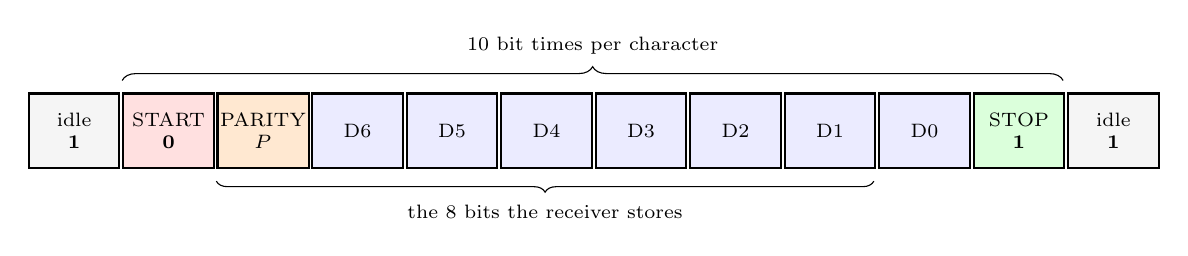
\begin{tikzpicture}[
  bit/.style={draw, minimum height=0.95cm, minimum width=1.15cm, align=center,
              font=\scriptsize, inner sep=1pt},
  >=Stealth, thick
]
  \node[bit, fill=black!4]   (i0) at (0,0)      {idle\\\textbf{1}};
  \node[bit, fill=red!12]    (st) at (1.2,0)    {START\\\textbf{0}};
  \node[bit, fill=orange!18] (pa) at (2.4,0)    {PARITY\\$P$};
  \node[bit, fill=blue!8]    (d6) at (3.6,0)    {D6};
  \node[bit, fill=blue!8]    (d5) at (4.8,0)    {D5};
  \node[bit, fill=blue!8]    (d4) at (6.0,0)    {D4};
  \node[bit, fill=blue!8]    (d3) at (7.2,0)    {D3};
  \node[bit, fill=blue!8]    (d2) at (8.4,0)    {D2};
  \node[bit, fill=blue!8]    (d1) at (9.6,0)    {D1};
  \node[bit, fill=blue!8]    (d0) at (10.8,0)   {D0};
  \node[bit, fill=green!14]  (sp) at (12.0,0)   {STOP\\\textbf{1}};
  \node[bit, fill=black!4]   (i1) at (13.2,0)   {idle\\\textbf{1}};

  \draw[decorate, decoration={brace, amplitude=5pt}, thin]
      (st.north west) ++(0,0.15) -- ++(11.95,0)
      node[midway, above=6pt, font=\scriptsize]{10 bit times per character};

  \draw[decorate, decoration={brace, mirror, amplitude=4pt}, thin]
      (pa.south west) ++(0,-0.15) -- ++(8.35,0)
      node[midway, below=5pt, font=\scriptsize]{the 8 bits the receiver stores};
\end{tikzpicture}
\end{latin}
\end{center}

دو تفاوت با \lr{UART} استاندارد وجود دارد و هر دو مستقیما از صورت آزمایش می‌آید:

\begin{enumerate}
  \item بیت توازن {قبل} از داده فرستاده می‌شود، نه بعد از آن. پیامد این انتخاب برای سخت‌افزار مهم است: فرستنده باید {تمام} کاراکتر را پیش از شروع ارسال در اختیار داشته باشد، چون توازن تابعی از همه‌ی هفت بیت است. به همین دلیل داده به‌صورت موازی بارگذاری می‌شود و توازن در همان لحظه‌ی بارگذاری به‌صورت ترکیبی محاسبه می‌شود.
  \item بار مفید ۷ بیت است و گیرنده ۸ بیت پس از بیت شروع را در یک ثبات ذخیره می‌کند.
\end{enumerate}

\subsubsection*{چرا داده \lr{MSB}‌اول فرستاده می‌شود}

در \lr{UART} استاندارد داده از کم‌ارزش‌ترین بیت شروع می‌شود. اینجا عمدا برعکس عمل شده است و دلیلش خواسته‌ی خود صورت آزمایش است: گیرنده باید ۸ بیت را در {یک ثبات ۸ بیتی} بریزد.

گیرنده یک ثبات لغزشی است که هر بیت جدید را از سمت کم‌ارزش وارد می‌کند. اگر ترتیب ارسال \lr{P, D6, D5, ..., D0} باشد، محتوای ثبات پس از هشت شیفت دقیقا این است:

\begin{center}
\lr{rx\_reg = \{P, D6, D5, D4, D3, D2, D1, D0\}}
\end{center}

یعنی بیت توازن در پرارزش‌ترین جایگاه و کد \lr{ASCII} بدون هیچ جابه‌جایی در هفت بیت پایین. اگر داده \lr{LSB}‌اول فرستاده می‌شد، همان ثبات کد \lr{ASCII} را {برعکس} نگه می‌داشت و برای استفاده از آن باید یک معکوس‌کننده‌ی بیتی اضافه می‌شد — منطقی که هیچ کاری جز جبران یک انتخاب بد نمی‌کند.

\subsubsection*{تولید نرخ بیت و نمونه‌برداری ۱۶ برابر}

هر واحد یک شمارنده‌ی تقسیم دارد که پالسی به نام \lr{os\_tick} با نرخ {۱۶ برابر} نرخ بیت تولید می‌کند. فرستنده و گیرنده‌ی یک واحد هر دو از همین یک پالس استفاده می‌کنند، پس هزینه‌ی هر \lr{UART} یک شمارنده است نه دو تا.

\begin{latin}
\begin{lstlisting}[style=verilog,numbers=none]
DIVISOR = f_clk / (16 * baud)      // synthesis: e.g. 50 MHz / (16 * 115200) = 27
\end{lstlisting}
\end{latin}

نسبت تقسیم پارامتر است تا در سنتز مقدار واقعی و در شبیه‌سازی مقداری کوچک استفاده شود؛ در غیر این صورت هر تست‌بنچ باید میلیون‌ها کلاک بی‌کار را شبیه‌سازی می‌کرد.

اما چرا اصلا ۱۶ برابر؟ چون گیرنده کلاک فرستنده را ندارد. تنها لنگرگاه زمانی‌اش لبه‌ی پایین‌رونده‌ی بیت شروع است و این لبه با دقت {یک پالس نمونه‌برداری} تشخیص داده می‌شود. با ۱۶ برابر، این خطای اولیه $\frac{1}{16}$ یک بیت است و نقطه‌ی نمونه‌برداری آن‌قدر به وسط بیت نزدیک می‌ماند که تا انتهای فریم هم داخل بیت درست باقی بماند. جزئیات این حاشیه‌ی خطا در بخش تست‌ها می‌آید.

\subsubsection*{فرستنده}

فرستنده یک ماشین حالت ساده است که هر حالت آن دقیقا $16$ پالس \lr{os\_tick} طول می‌کشد:

\begin{center}
\begin{latin}
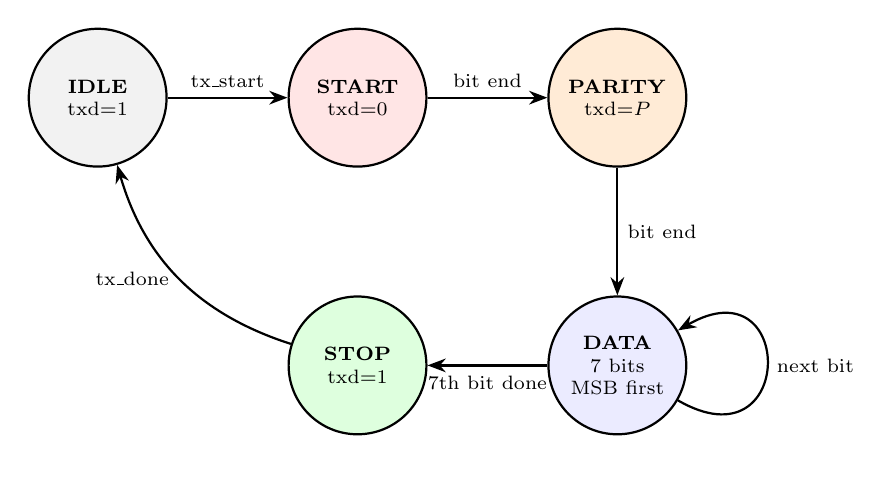
\begin{tikzpicture}[
  st/.style={draw, circle, minimum size=1.75cm, align=center, font=\scriptsize, inner sep=1pt},
  >=Stealth, thick
]
  \node[st, fill=black!5]    (idle) at (0,0)     {\textbf{IDLE}\\txd=1};
  \node[st, fill=red!10]     (start) at (3.3,0)  {\textbf{START}\\txd=0};
  \node[st, fill=orange!16]  (par) at (6.6,0)    {\textbf{PARITY}\\txd=$P$};
  \node[st, fill=blue!8]     (data) at (6.6,-3.4){\textbf{DATA}\\7 bits\\MSB first};
  \node[st, fill=green!13]   (stop) at (3.3,-3.4){\textbf{STOP}\\txd=1};

  \draw[->] (idle) -- node[midway,above,font=\scriptsize]{tx\_start} (start);
  \draw[->] (start) -- node[midway,above,font=\scriptsize]{bit end} (par);
  \draw[->] (par) -- node[midway,right,font=\scriptsize]{bit end} (data);
  \draw[->] (data) -- node[midway,below,font=\scriptsize]{7th bit done} (stop);
  \draw[->] (stop) to[bend left=28] node[midway,left,font=\scriptsize]{tx\_done} (idle);
  \draw[->] (data) to[out=-30,in=30,looseness=5]
      node[midway,right,font=\scriptsize]{next bit} (data);
\end{tikzpicture}
\end{latin}
\end{center}

دو نکته‌ی پیاده‌سازی:

\textbf{بیت شروع در همان لبه‌ی بارگذاری روی خط می‌رود.} اگر منتظر اولین \lr{os\_tick} می‌ماندیم، اولین بیت به اندازه‌ی فاز باقی‌مانده‌ی شمارنده کش می‌آمد. با پایین بردن فوری خط و {صفر کردن هم‌زمان شمارنده‌ی داخل بیت}، طول بیت شروع دقیقا $16$ پالس می‌شود و همه‌ی بیت‌های بعدی هم به همان اندازه.

\textbf{درخواست جدید در میانه‌ی فریم نادیده گرفته می‌شود، نه صف.} سیگنال \lr{tx\_busy} برای همین بیرون داده شده است. اگر درخواست‌ها صف می‌شدند، به یک بافر نیاز بود؛ و اگر فریم جاری را قطع می‌کردند، گیرنده‌ی طرف مقابل یک فریم ناقص می‌دید. این رفتار در تست‌بنچ صریحا بررسی شده است.

\begin{latin}
\lstinputlisting[style=verilog]{../rtl/uart_tx.v}
\end{latin}

\subsubsection*{گیرنده}

گیرنده کار سختی دارد: باید بدون کلاک مشترک بفهمد هر بیت کجا شروع و کجا تمام می‌شود.

\begin{center}
\begin{latin}
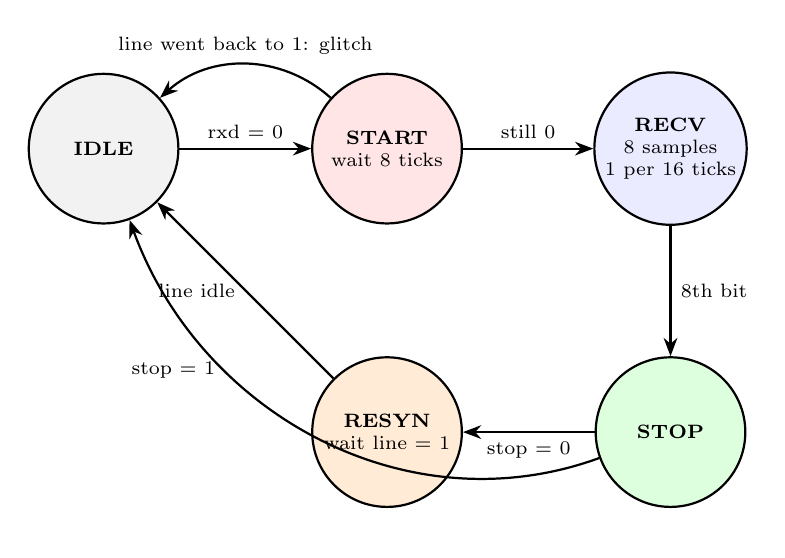
\begin{tikzpicture}[
  st/.style={draw, circle, minimum size=1.9cm, align=center, font=\scriptsize, inner sep=1pt},
  >=Stealth, thick
]
  \node[st, fill=black!5]   (idle)  at (0,0)      {\textbf{IDLE}};
  \node[st, fill=red!10]    (start) at (3.6,0)    {\textbf{START}\\wait 8 ticks};
  \node[st, fill=blue!8]    (recv)  at (7.2,0)    {\textbf{RECV}\\8 samples\\1 per 16 ticks};
  \node[st, fill=green!13]  (stop)  at (7.2,-3.6) {\textbf{STOP}};
  \node[st, fill=orange!16] (res)   at (3.6,-3.6) {\textbf{RESYN}\\wait line = 1};

  \draw[->] (idle) -- node[midway,above,font=\scriptsize]{rxd = 0} (start);
  \draw[->] (start) -- node[midway,above,font=\scriptsize]{still 0} (recv);
  \draw[->] (start) to[bend right=42]
      node[midway,above,font=\scriptsize]{line went back to 1: glitch} (idle);
  \draw[->] (recv) -- node[midway,right,font=\scriptsize]{8th bit} (stop);
  \draw[->] (stop) -- node[midway,below,font=\scriptsize]{stop = 0} (res);
  \draw[->] (res) -- node[midway,left,font=\scriptsize]{line idle} (idle);
  \draw[->] (stop) to[out=200,in=-70]
      node[pos=0.7,left,font=\scriptsize]{stop = 1} (idle);
\end{tikzpicture}
\end{latin}
\end{center}

\textbf{الف) هم‌گام‌سازی ورودی.} خط سریال از دامنه‌ی زمانی دیگری (یا روی برد، از یک پایه) می‌آید و نباید مستقیم به ماشین حالت وصل شود. دو فلیپ‌فلاپ پشت سر هم احتمال \lr{metastability} را عملا از بین می‌برند.

\textbf{ب) رد کردن نویز به جای شروع فریم.} با پایین آمدن خط، گیرنده {نیم بیت} صبر می‌کند و دوباره خط را می‌بیند. اگر خط بالا رفته باشد، آنچه دیده شده یک سوزن نویزی بوده و گیرنده به \lr{IDLE} برمی‌گردد. اگر هنوز پایین باشد، این واقعا بیت شروع است — و از قضا این لحظه دقیقا {وسط} بیت شروع است.

\textbf{ج) نمونه‌برداری از وسط هر بیت.} از همان نقطه به بعد، هر $16$ پالس یک بار نمونه گرفته می‌شود. چون نقطه‌ی شروع وسط بیت شروع بود، همه‌ی نمونه‌های بعدی هم دقیقا وسط بیت خودشان می‌افتند — بیشترین فاصله‌ی ممکن از هر دو لبه، یعنی بیشترین تحمل نسبت به اختلاف نرخ بیت دو طرف.

\textbf{د) بازگشت به هم‌گامی پس از خطای فریم.} اگر بیت خاتمه صفر خوانده شود، فریم خراب بوده و خط هنوز پایین است. برگشتن مستقیم به \lr{IDLE} یعنی همان صفر بلافاصله به‌عنوان بیت شروع بعدی تفسیر شود و یک فریم زباله‌ی دیگر تولید کند. به همین دلیل حالت \lr{RESYN} اضافه شده که تا بی‌کار شدن خط منتظر می‌ماند. این رفتار هم در تست‌بنچ بررسی شده است.

\begin{latin}
\lstinputlisting[style=verilog]{../rtl/uart_rx.v}
\end{latin}

\subsubsection*{اتصال دو واحد}

خواسته‌ی پایانی صورت آزمایش این است که دو واحد به یکدیگر وصل شوند. ماژول \lr{uart\_link} دقیقا همین است: خروجی فرستنده‌ی هر واحد به ورودی گیرنده‌ی واحد دیگر می‌رود و این دو سیم تمام «کابل» بین دو دستگاه‌اند.

\begin{center}
\begin{latin}
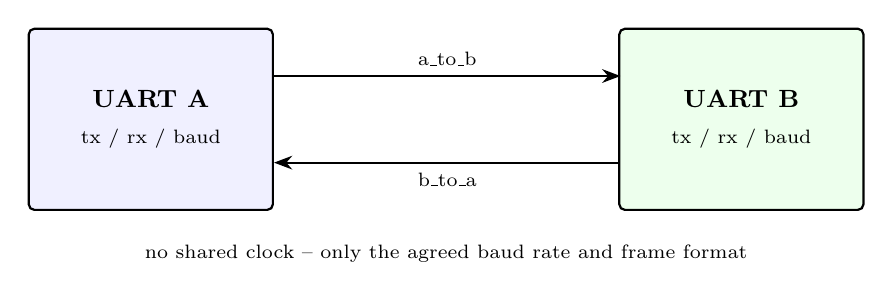
\begin{tikzpicture}[
  box/.style={draw, rounded corners=2pt, minimum height=2.3cm, minimum width=3.1cm,
              align=center, font=\small},
  >=Stealth, thick
]
  \node[box, fill=blue!6]  (a) at (0,0)   {\textbf{UART A}\\[2pt]\scriptsize tx / rx / baud};
  \node[box, fill=green!7] (b) at (7.5,0) {\textbf{UART B}\\[2pt]\scriptsize tx / rx / baud};

  \draw[->] (a.east) ++(0,0.55) -- ++(4.4,0)
      node[midway, above, font=\scriptsize]{a\_to\_b};
  \draw[<-] (a.east) ++(0,-0.55) -- ++(4.4,0)
      node[midway, below, font=\scriptsize]{b\_to\_a};

  \node[font=\scriptsize, align=center] at (3.75,-1.7)
      {no shared clock -- only the agreed baud rate and frame format};
\end{tikzpicture}
\end{latin}
\end{center}

دو واحد پارامتر تقسیم {جداگانه} دارند. با مقادیر برابر، لینک کاملا هم‌نرخ است؛ با مقادیر کمی متفاوت، دو بردی مدل می‌شوند که کریستال‌هایشان با هم اختلاف دارند — و این دقیقا همان چیزی است که نمونه‌برداری ۱۶ برابر باید از پس آن بربیاید.

\begin{latin}
\lstinputlisting[style=verilog]{../rtl/uart_link.v}
\end{latin}

\subsubsection*{شکل موج}

\begin{center}
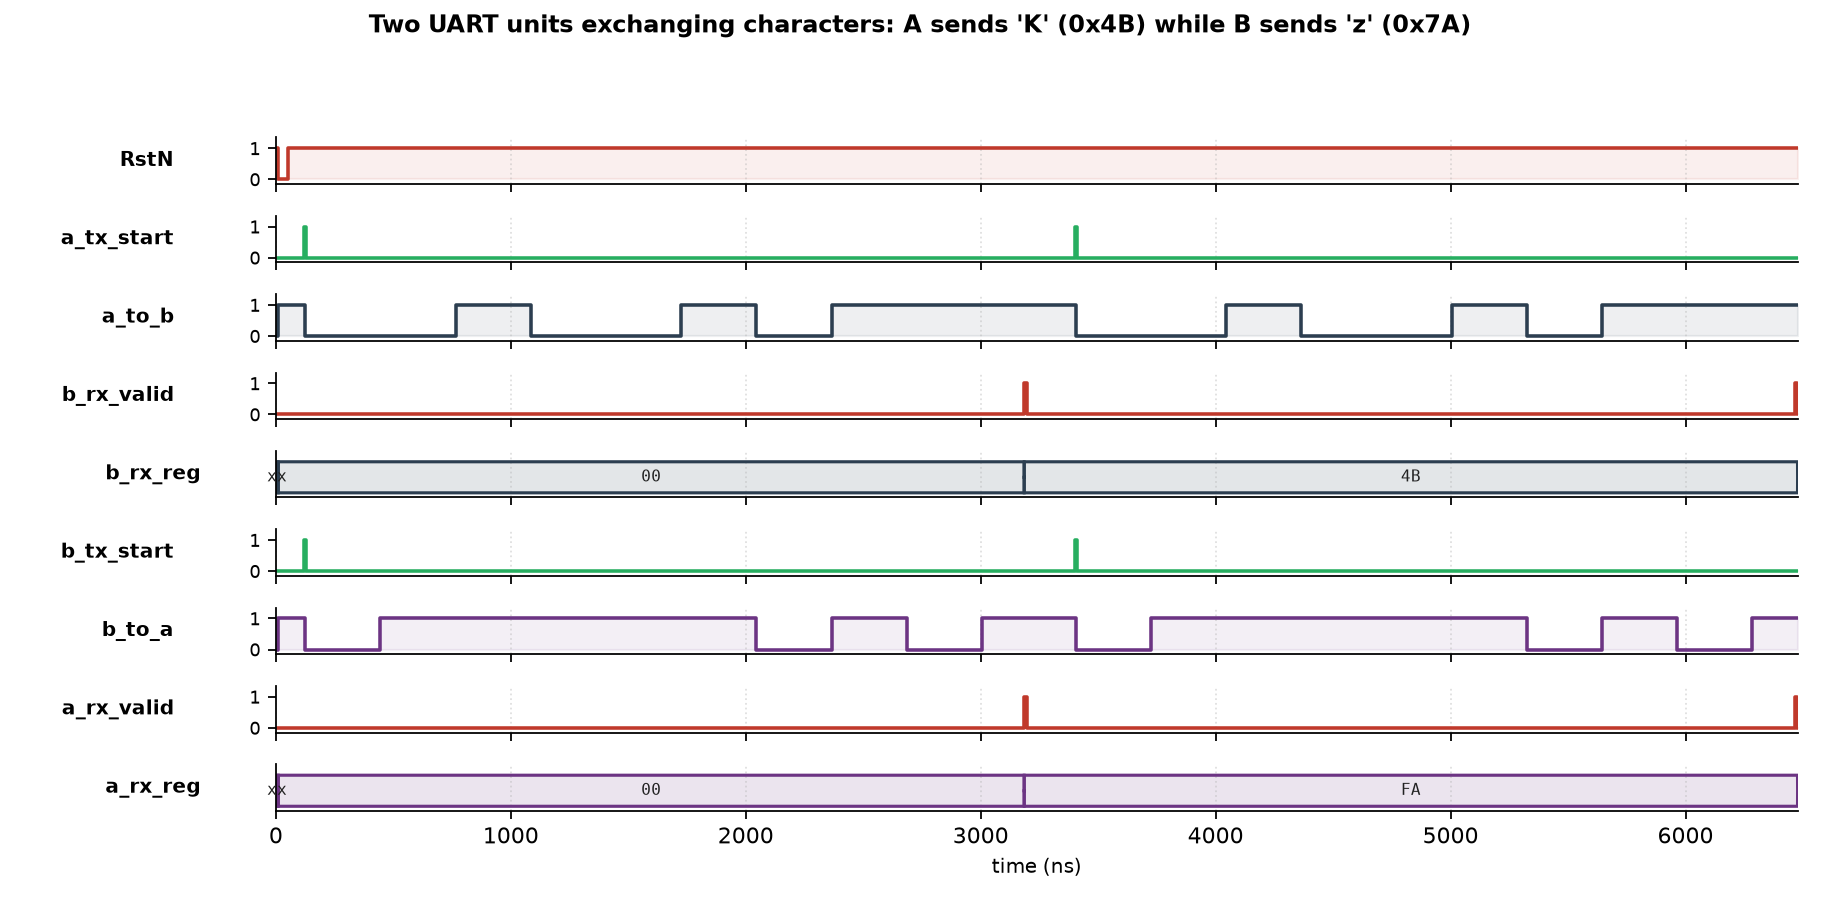
\includegraphics[width=\textwidth]{figs/wave_uart.png}\\[0.4em]
\end{center}

در این شکل‌موج، واحد \lr{A} کاراکتر \lr{'K'} (کد \lr{0x4B}) و واحد \lr{B} در همان لحظه کاراکتر \lr{'z'} (کد \lr{0x7A}) را می‌فرستد. دو سیم \lr{a\_to\_b} و \lr{b\_to\_a} هم‌زمان مشغول‌اند، یعنی لینک واقعا {دوطرفه‌ی هم‌زمان} است.

مقادیر ذخیره‌شده در ثبات‌ها نشان می‌دهد ترتیب بیت‌ها درست است:

\begin{center}
\begin{tabular}{@{}llll@{}}
\toprule
{کاراکتر} & {کد \lr{ASCII}} & {توازن زوج} & {محتوای ثبات ۸ بیتی} \\
\midrule
\lr{'K'} & \lr{0x4B} = \lr{1001011} & $0$ & \lr{0\_1001011} = \lr{0x4B} \\
\lr{'z'} & \lr{0x7A} = \lr{1111010} & $1$ & \lr{1\_1111010} = \lr{0xFA} \\
\bottomrule
\end{tabular}
\end{center}

توجه کنید که برای \lr{'K'} تعداد یک‌ها زوج است پس بیت توازن صفر می‌شود و محتوای ثبات با خود کد \lr{ASCII} یکی درمی‌آید؛ برای \lr{'z'} تعداد یک‌ها فرد است، بیت توازن یک می‌شود و در پرارزش‌ترین جایگاه ثبات می‌نشیند. در هر دو حالت هفت بیت پایین ثبات بدون هیچ پردازش اضافه همان کد \lr{ASCII} است — همان چیزی که در بخش ترتیب بیت‌ها درباره‌اش صحبت شد.

\subsubsection*{تست‌بنچ‌ها}

\begin{center}
\begin{tabular}{@{}l p{9.2cm}@{}}
\toprule
{تست‌بنچ} & {روش} \\
\midrule
\lr{tb\_uart\_tx}   & الگوی ۱۰ بیتی مورد انتظار را {از روی صورت آزمایش} می‌سازد و خط را وسط هر بیت نمونه‌برداری می‌کند \\
\lr{tb\_uart\_rx}   & فریم‌ها را بیت‌به‌بیت {از داخل خود تست‌بنچ} روی خط می‌راند \\
\lr{tb\_uart\_link} & تنها جایی که دو ماژول با هم کار می‌کنند؛ اینجا هدف بررسی {مبادله} است نه قالب فریم \\
\bottomrule
\end{tabular}
\end{center}

\textbf{تست فرستنده} هر ۱۲۸ کد \lr{ASCII} را با هر دو قرارداد توازن زوج و فرد می‌فرستد و هر ۱۰ بیت هر فریم را جداگانه بررسی می‌کند. علاوه بر آن: بی‌کار بودن خط روی مقدار یک، درست بودن \lr{tx\_busy} در طول فریم، پالس \lr{tx\_done} در انتها، و نادیده گرفته شدن درخواست ارسال در میانه‌ی فریم.

\begin{latin}
\lstinputlisting[style=verilog]{../tb/tb_uart_tx.v}
\end{latin}

\textbf{تست گیرنده} همان ۱۲۸ کد را با هر دو قرارداد توازن روی خط می‌راند و علاوه بر آن چهار وضعیت غیرعادی را می‌سازد: بیت توازن خراب، بیت خاتمه‌ی گم‌شده، یک سوزن کوتاه روی خط، و فریم‌های پشت سر هم بدون هیچ فاصله‌ی بی‌کاری.

نکته‌ی ظریفی که این تست روشن می‌کند: پس از خطای توازن، داده {همچنان} در ثبات می‌نشیند و فقط پرچم خطا بالا می‌رود. تصمیم درباره‌ی دور انداختن یا نینداختن کاراکتر خراب کار لایه‌ی بالاتر است، نه کار \lr{UART}.

\begin{latin}
\lstinputlisting[style=verilog]{../tb/tb_uart_rx.v}
\end{latin}

\textbf{تست لینک} دو سناریو دارد. در اولی دو واحد کاملا هم‌نرخ‌اند و هر ۱۲۸ کاراکتر {هم‌زمان در هر دو جهت} رد و بدل می‌شود (واحد \lr{A} کاراکتر و واحد \lr{B} مکمل بیتی همان کاراکتر را می‌فرستد تا دو جهت هرگز الگوی یکسان حمل نکنند).

در دومی نسبت تقسیم دو واحد $20$ و $21$ گرفته شده است، یعنی اختلاف نرخ بیت $5\%$. این عدد اتفاقی نیست؛ درست زیر حد نظری قرار دارد. آخرین بیتی که گیرنده نمونه می‌گیرد بیت خاتمه است که $9.5$ بیت پس از نقطه‌ی هم‌گامی قرار دارد و نمونه تا وقتی درست است که رانش انباشته از نصف بیت بیشتر نشود:

\[
\text{حد اختلاف نرخ} \;=\; \frac{0.5}{9.5} \;\approx\; 5.3\%
\]

این حد به‌صورت تجربی هم اندازه‌گیری شد: با جاروب چند لینک با اختلاف‌های مختلف، تا $5\%$ همه‌ی کاراکترها سالم می‌رسند و از $6\%$ به بعد هیچ‌کدام نمی‌رسند. یعنی مدار واقعا به همان حدی می‌رسد که تئوری می‌گوید، نه کمتر.

\begin{latin}
\lstinputlisting[style=verilog]{../tb/tb_uart_link.v}
\end{latin}

\subsubsection*{اندازه‌گیری نقطه‌ی نمونه‌برداری}

ادعای «نمونه‌برداری از وسط بیت» چیزی است که به‌راحتی می‌شود نوشت و اشتباه پیاده‌سازی کرد، چون یک نمونه‌ی کمی دور از وسط هم در لینک هم‌نرخ کاملا درست کار می‌کند و هیچ تستی را رد نمی‌کند. تنها اثرش این است که حاشیه‌ی تحمل اختلاف نرخ بی‌سروصدا کم می‌شود.

بنابراین نقطه‌ی نمونه‌برداری مستقیما اندازه‌گیری شد: شمارش پالس‌های \lr{os\_tick} از لحظه‌ی پایین آمدن خط تا لحظه‌ای که هر بیت در ثبات می‌نشیند. نقاط ایده‌آل $8$، $24$، $40$، \ldots هستند.

اولین اندازه‌گیری اعداد $26$، $42$، $58$، \ldots را داد؛ یعنی هر نمونه {دو تیک} دیرتر از وسط بیت گرفته می‌شد. علتش یک خطای واحد در شمارنده‌ی نیم‌بیت بود:

\begin{latin}
\begin{lstlisting}[style=verilog,numbers=none]
if (os == OS/2)      // wrong: os starts at 0 and is tested BEFORE
                     // incrementing, so this waits OS/2 + 1 ticks
if (os == OS/2 - 1)  // right: counting 0..OS/2-1 is exactly OS/2 ticks
\end{lstlisting}
\end{latin}

پس از اصلاح، اعداد به $25$، $41$، $57$، \ldots رسیدند. یک تیک باقی‌مانده اجتناب‌ناپذیر است: شمارنده‌ی داخل بیت فقط روی مرز پالس‌های نمونه‌برداری می‌تواند شروع شود، پس تا $\frac{1}{16}$ بیت خطای اولیه همیشه وجود دارد — همان چیزی که در تحلیل حاشیه‌ی خطا هم لحاظ شده است.

اثر این یک تیک کم نیست: پیش از اصلاح، لینک با اختلاف نرخ $5\%$ کاراکتر گم می‌کرد و اکنون نمی‌کند.

\subsubsection*{نتایج تست}

\begin{latin}
\lstinputlisting[basicstyle=\ttfamily\scriptsize]{figs/test_run_output.txt}
\end{latin}

\pagebreak
\subsubsection*{خروجی سنتز (\lr{Quartus Prime})}

طرح روی \lr{Intel Quartus Prime Lite Edition 21.1.0} با موجودیت سطح‌بالای \lr{uart\_link} (دو نمونه‌ی \lr{uart} در \lr{uart\_link}) سنتز و Place \& Route شد. دستگاه هدف: \lr{Cyclone V} (\lr{5CGXFC7C7F23C8}).

\begin{center}
\begin{tabular}{@{}lr@{}}
\toprule
{مورد} & {نتیجه} \\
\midrule
وضعیت کامپایل & موفق ($0$ خطا، $14$ هشدار) \\
\lr{Logic utilization (ALMs)} & $96 / 56480$ ($<1\%$) \\
\lr{Total registers} & $150$ \\
\lr{Total pins} & $60 / 268$ ($22\%$) \\
\lr{Block memory bits} & $0$ \\
\lr{DSP Blocks} & $0$ \\
\lr{Worst-case setup slack} & $-0.674$ \\
\lr{Worst-case hold slack} & $+0.166$ \\
\lr{Min pulse width slack} & $-0.091$ \\
\bottomrule
\end{tabular}
\end{center}

\begin{center}

\includegraphics[width=\textwidth]{figs/quartus_synthesis.jpg}
\end{center}

\end{document}
